%%%%%%%%%%%%%%%%%%%%%%%%%%%%%%%%%%%%%%%%%%%%%%%%%%%%%%%%%%%%%%%%%%%%%%%%%%%%%%%%%%%%%
% PACOTES                                                                           %
%%%%%%%%%%%%%%%%%%%%%%%%%%%%%%%%%%%%%%%%%%%%%%%%%%%%%%%%%%%%%%%%%%%%%%%%%%%%%%%%%%%%%
\documentclass[a4paper,11pt]{amsart}

%-----------------------------------------------------------------------------------%
% LAYOUT DA PÁGINA                                                                  %
%-----------------------------------------------------------------------------------%
\usepackage[top=2.25cm, bottom=2.25cm, left=2.25cm, right=2.25cm]{geometry}
%\usepackage{fancyhdr} % Permite controlar como são exibidos os cabeçalhos

%-----------------------------------------------------------------------------------%
% FORMATAÇÃO DO TEXTO                                                               %
%-----------------------------------------------------------------------------------%
%\usepackage{setspace} % Permite definir o espaçamento entre linhas

%-----------------------------------------------------------------------------------%
% PACOTES DE IMAGENS                                                                %
%-----------------------------------------------------------------------------------%
\usepackage[pdftex]{graphicx}
\pdfsuppresswarningpagegroup=1 % A warning issued when several PDF images are
% imported in the same page. Mostly harmless, can be almost always supressed.
%\usepackage[pstarrows]{pict2e} % Amplia as funcionalidades do ambiente picture
\usepackage{tikz}
\usetikzlibrary{shapes, arrows, arrows.meta, positioning}

%-----------------------------------------------------------------------------------%
% PACOTES DE TABELAS                                                                %
%-----------------------------------------------------------------------------------%
\usepackage{array} % Facilita a formatação de tabelas
%\usepackage{multirow} % Permite criar células que ocupam várias linhas em uma tabela
\usepackage{longtable} % Permite criar tabelas que quebram de página

%-----------------------------------------------------------------------------------%
% PACOTES MATEMÁTICOS DE BASE                                                       %
%-----------------------------------------------------------------------------------%
\usepackage{amsfonts,amstext,amscd,bezier,amsthm,amssymb}
\usepackage[centertags]{amsmath}

%-----------------------------------------------------------------------------------%
% PACOTES DE SÍMBOLOS MATEMÁTICOS                                                   %
%-----------------------------------------------------------------------------------%
\usepackage{mathtools} % Símbolos matemáticos extras. (ex.: \xrightharpoon)
%\usepackage[integrals]{wasysym} % Muda o estilo das integrais, além de outros
%                                 símbolos extras
%\usepackage[nice]{nicefrac} % Permite o uso de frações "melhores". Usar \nicefrac{}{}

%-----------------------------------------------------------------------------------%
% PACOTES DE FONTES MATEMÁTICAS                                                     %
%-----------------------------------------------------------------------------------%
%\usepackage{mathbbol} % Quase todos os símbolos com \mathbb
%\usepackage{bbm} % Extensão dos símbolos de \mathbb. Usar comando \mathbbm
%\usepackage{calrsfs} % Muda o estilo de \mathcal
%\usepackage[mathcal]{euscript} % Muda o estilo de \mathcal

%-----------------------------------------------------------------------------------%
% PACOTES DE CODIFICAÇÃO DE FONTES                                                  %
%-----------------------------------------------------------------------------------%
\usepackage[utf8]{inputenc} % Permite o uso de caracteres ISO 8859-1, incluindo os
%                               caracteres acentuados diretamente.
\usepackage[T1]{fontenc} % Uso de fontes T1, necessário para tratar caracteres
%                          acentuados como um único bloco.

%-----------------------------------------------------------------------------------%
% PACOTES DE LÍNGUAS                                                                %
%-----------------------------------------------------------------------------------%
\usepackage[french]{babel} % Seleciona a língua do documento, definindo nomes de
%                              seções, nome do índice, da bibliografia, etc. Em caso
%                              de documento com mais de uma língua, a padrão é a
%                              última.
\NoAutoSpaceBeforeFDP % Utilizar em francês se quiser evitar espaços antes de :

%-----------------------------------------------------------------------------------%
% PACOTES DE BIBLIOGRAFIA                                                           %
%-----------------------------------------------------------------------------------%
%\usepackage{babelbib} % Permite definir a língua das entradas da bibliografia. Usar
%                       [fixlanguage] para uma mesma língua para todas as entradas e
%                       \selectbiblanguage{} para definir a língua. Um estilo compa-
%                       tível com babelbib deve ser usado (ex: babplain)
\usepackage{cite} % Organiza os elementos citados dentro de um mesmo \cite.

%-----------------------------------------------------------------------------------%
% PACOTES DE FONTES                                                                 %
%-----------------------------------------------------------------------------------%
% Computer Modern (fonte padrão)                                                    %
% - - - - - - - - - - - - - - - - - - - - - - - - - - - - - - - - - - - - - - - - - %
%\usepackage{ae} % A usar com a fonte padrão do LaTeX quando forem gerados PDFs, para
%                 corrigir erros de visualização

% Computer Modern Bright (sans serif)                                               %
% - - - - - - - - - - - - - - - - - - - - - - - - - - - - - - - - - - - - - - - - - %
%\usepackage{cmbright}

% Times New Roman                                                                   %
% - - - - - - - - - - - - - - - - - - - - - - - - - - - - - - - - - - - - - - - - - %
%\usepackage{mathptmx} % Muda texto e modo matemático
%\usepackage{times} % Apenas texto, não muda modo matemático

% Arial                                                                             %
% - - - - - - - - - - - - - - - - - - - - - - - - - - - - - - - - - - - - - - - - - %
%\usepackage[scaled]{uarial} % Arial como fonte sans serif padrão

% Palatino                                                                          %
% - - - - - - - - - - - - - - - - - - - - - - - - - - - - - - - - - - - - - - - - - %
%\usepackage{mathpazo} % Muda texto e modo matemático
%\usepackage{palatino} % Apenas texto, não muda modo matemático

% Concrete                                                                          %
% - - - - - - - - - - - - - - - - - - - - - - - - - - - - - - - - - - - - - - - - - %
%\usepackage{ccfonts} % Texto: Concrete; Matemático: Concrete Math
%\usepackage{ccfonts, eulervm} % Texto: Concrete; Matemático: Euler

% Iwona                                                                             %
% - - - - - - - - - - - - - - - - - - - - - - - - - - - - - - - - - - - - - - - - - %
%\usepackage[math]{iwona} % Texto e modo matemático: Iwona

% Kurier                                                                            %
% - - - - - - - - - - - - - - - - - - - - - - - - - - - - - - - - - - - - - - - - - %
%\usepackage[math]{kurier} % Texto e modo matemático: Kurier

% Antykwa Póltawskiego                                                              %
% - - - - - - - - - - - - - - - - - - - - - - - - - - - - - - - - - - - - - - - - - %
%\usepackage{antpolt} % Texto: Antykwa Póltawskiego; Matemático: nenhum
                     % Usar fontenc = QX ou OT4

% Utopia                                                                            %
% - - - - - - - - - - - - - - - - - - - - - - - - - - - - - - - - - - - - - - - - - %                     
%\usepackage{fourier} % Texto: Utopia; Matemático: Fourier

% KP Serif                                                                          %
% - - - - - - - - - - - - - - - - - - - - - - - - - - - - - - - - - - - - - - - - - %
\usepackage{kpfonts}

%-----------------------------------------------------------------------------------%
% CORES                                                                             %
%-----------------------------------------------------------------------------------%
\usepackage{color}
\definecolor{darkgreen}{rgb}{0,0.5,0}
\definecolor{darkmagenta}{rgb}{0.5,0,0.5}
\definecolor{darkgray}{rgb}{0.5,0.5,0.5}
\definecolor{darkblue}{rgb}{0.2,0.2,0.4}
\definecolor{darkred}{rgb}{0.6,0.15,0.15}
\definecolor{gray}{rgb}{0.65,0.65,0.65}
\definecolor{lightgray}{rgb}{0.8,0.8,0.8}
\definecolor{lightblue}{rgb}{0.5,0.5,1}
\definecolor{lightgreen}{rgb}{0.5,1,0.5}
\definecolor{deadred}{rgb}{0.7, 0.2, 0.2}
\definecolor{deadblue}{rgb}{0.2, 0.2, 0.7}

%-----------------------------------------------------------------------------------%
% PACOTES DIVERSOS                                                                  %
%-----------------------------------------------------------------------------------%
\usepackage{icomma} % Permite uso de vírgula como separador decimal
\usepackage{url} % Pacote para não ter problemas com URLs. Usar \url{}
%\usepackage{randtext} % Troca a ordem de letras de uma frase (útil com e-mails em
                      % PDFs a serem publicados on-line.
\usepackage[hidelinks]{hyperref}
%\usepackage{showkeys} % Para mostrar o nome dos labels
\usepackage{enumitem} % Facilita o uso de listas, inclusive referências a itens de
                      % listas.
%\usepackage[absolute]{textpos} % Posição absoluta de texto na página
%\usepackage{pdfpages} % Permite incluir documentos em PDF no arquivo
%\usepackage{refcheck} % Verifica as referências procurando por
%                      % labels não usados ou equações numeradas sem labels.
%                      % Verificar o arquivo .log e procurar por RefCheck.
\usepackage[french, onelanguage]{algorithm2e}

%%%%%%%%%%%%%%%%%%%%%%%%%%%%%%%%%%%%%%%%%%%%%%%%%%%%%%%%%%%%%%%%%%%%%%%%%%%%%%%%%%%%%
% CONFIGURAÇÕES                                                                     %
%%%%%%%%%%%%%%%%%%%%%%%%%%%%%%%%%%%%%%%%%%%%%%%%%%%%%%%%%%%%%%%%%%%%%%%%%%%%%%%%%%%%%

%-----------------------------------------------------------------------------------%
% FORMATAÇÃO DO TEXTO                                                               %
%-----------------------------------------------------------------------------------%
%\onehalfspacing % Espaçamento 1 1/2 (definido no pacote setspace)

%-----------------------------------------------------------------------------------%
% DEFINIÇÃO DE AMBIENTES MATEMÁTICOS                                                %
%-----------------------------------------------------------------------------------%
\theoremstyle{plain}
\newtheorem*{prop}{Proposition}

%-----------------------------------------------------------------------------------%
% DEFINIÇÃO DE COMANDOS MATEMÁTICOS                                                 %
%-----------------------------------------------------------------------------------%
%\newcommand*\diff{\mathop{}\!\mathrm{d}}

%\newcommand{\norm}[1]{\left\lVert #1\right\lVert} % Norma
%\newcommand{\abs}[1]{\left\lvert #1\right \rvert} % Valor absoluto
%\newcommand{\floor}[1]{\left\lfloor #1 \right\rfloor} % Arredondar para baixo
%\newcommand{\ceil}[1]{\left\lceil #1 \right\rceil} % Arredondar para cima
\DeclarePairedDelimiter{\ceil}{\lceil}{\rceil}
\DeclarePairedDelimiter{\floor}{\lfloor}{\rfloor}
\DeclarePairedDelimiter{\abs}{\lvert}{\rvert}
\DeclareMathOperator*{\argmax}{argmax}

%-----------------------------------------------------------------------------------%
% NUMERAÇÃO DE ELEMENTOS                                                            %
%-----------------------------------------------------------------------------------%
%\numberwithin{table}{section}
%\numberwithin{table}{subsection}
%\numberwithin{figure}{section}
%\numberwithin{figure}{subsection}
%\numberwithin{equation}{section}
%\numberwithin{equation}{subsection}
%\numberwithin{theo}{chapter}
%\numberwithin{theo}{subsection}

% Maximal percentage of the page occupied by floats
\renewcommand\floatpagefraction{.9}
\renewcommand\topfraction{.9}
\renewcommand\bottomfraction{.9}
\renewcommand\textfraction{.1}
% Maximal number of floats per page
\setcounter{totalnumber}{50}
\setcounter{topnumber}{50}
\setcounter{bottomnumber}{50}

%%%%%%%%%%%%%%%%%%%%%%%%%%%%%%%%%%%%%%%%%%%%%%%%%%%%%%%%%%%%%%%%%%%%%%%%%%%%%%%%%%%%%
% ESTRUTURA DO DOCUMENTO                                                            %
%%%%%%%%%%%%%%%%%%%%%%%%%%%%%%%%%%%%%%%%%%%%%%%%%%%%%%%%%%%%%%%%%%%%%%%%%%%%%%%%%%%%%
\begin{document}

\setlist[itemize]{label=\textbullet, nosep, leftmargin = 0pt, listparindent = 0pt}

\pagestyle{plain}

\title{Compte Rendu TME6}
\author{CARNIELLI Ariana 3525837 \\
QUABOUL Dorian 3872944
}
\maketitle

\section*{Exercice 1}

\begin{itemize}
\item $Kp \to \lnot K \lnot Kp$

\texttt{imp nec P not nec not nec P} 

Toutes les feuilles sont ouvertes donc la formule est satisfiable. On teste si la formule est valide en vérifiant la négation de la formule : \texttt{not imp nec P not nec not nec P}. Comme toutes les feuilles sont fermées alors la formule originale est valide.

\item $Kp \land K K \lnot p$

\texttt{and nec P nec nec not P}

Toutes les feuilles sont fermées donc la formule est insatisfiable.

\item $Kp \to K K \lnot p$

\texttt{imp nec P nec nec not P}

La formule est satisfiable car les feuilles sont ouvertes. On teste si la formule est valide en vérifiant la négation de la formule :  \texttt{not imp nec P nec nec not P}. En regardant la négation de la formule on voit que toutes les feuilles sont ouvertes, donc la formule n'est que satisfiable et pas valide.
\end{itemize}

\section*{Exercice 2}

Pour montrer que l'équivalence donnée est valide dans un système, on la nie et on vérifie que cette négation est insatisfiable. On a alors : \texttt{not and imp not nec P nec not nec P imp nec not nec P not nec P}.

Lorsqu'on se place dans le système S4, on remarque qu'un des prémodèles est réalisable et donc que la formule originale n'est pas valide.

On sait que la formule est valide en S5 (KT45) car il y a une règle en plus qui correspond à l'euclidiannité. Donc on essaie de prouver que si on rajoute la règle d'euclidiannité en S4 la formule devient valide.

En effet, dans le prémodèle crée pour la négation de la formule en S4, nous avons un monde $w_1$ qui pointe vers 2 mondes $w_2$ et $w_3$. Donc la règle d'euclidiannité donnerait un lien entre $w_2$ et $w_3$ qui n'existe pas. Dans le monde $w_2$, il y a $\Box P$ et dans le monde $w_3$ il y a $\lnot P$ donc avec ce nouveau lien rajouté on obtiendrait un $P$ dans $w_3$ donc il y aurait une contradiction. Tous les prémodèles générés par la méthode des tableaux pour la négation de la formule avec l'euclidiannité sont insatisfiables donc la formule devient valide.

\section*{Exercice 3}

\section*{Exercice 4}

Dans la Figure~\ref{FigModele} on peut voir une façon d'étiqueter toutes les relations d'accessibilité par les agents 1, 2 et 3 de façon que les formules données à l'énoncé soient toutes valides et en satisfaisant la logique S5 (les relations de réflexivité ne sont pas dessinées mais sont prises en compte).

\begin{figure}[ht]
\centering
\begin{tikzpicture}
\node[draw, circle, thick] (w1) at (0, 0) {$w_1$};
\node at (0, 0.8) {$b, c$};
\node[draw, circle, thick] (w2) at (3, 0) {$w_2$};
\node at (3, 0.8) {$a, b$};
\node[draw, circle, thick] (w3) at (0, -3) {$w_3$};
\node at (0, -3.8) {$a$};
\node[draw, circle, thick] (w4) at (3, -3) {$w_4$};
\node at (3, -3.8) {$c$};
\draw[semithick] (w1) -- node[midway, above] {1, 2} (w2);
\draw[semithick] (w1) -- node[midway, left] {3} (w3);
\draw[semithick] (w2) -- node[midway, right] {3} (w4);
\draw[semithick] (w3) -- node[midway, below] {1} (w4);
\end{tikzpicture}
\caption{Réponse à l'exercice 4.}
\label{FigModele}
\end{figure}

On remarque que chaque formule ne porte que sur un seul agent. Pour la première formule, il faut que dans tous les mondes l'agent 3 ne sache pas si $b$, donc il faut que depuis tout monde il y ait un monde accessible avec $b$ et un monde accessible avec $\lnot b$. En particulier, pour que cela soit vrai dans $w_1$, il faut le relier à $w_3$ et, pour que ce soit vrai dans $w_2$, il faut le relier à $w_4$. Ces deux relations suffisent pour que cette formule soit valide dans tout monde.

Pour la deuxième formule, l'agent 1 ne peut pas savoir $c$ et il doit savoir si $b$. Pour qu'il ne sache pas $c$, il faut que $w_1$ soit relié à un autre monde qui n'a pas $c$, et de même pour $w_4$. Si on reliait $w_1$ à $w_3$, l'agent 2 ne saurait pas si $b$ dans le monde $w_1$, donc la seule possibilité est de relier $w_1$ à $w_2$. De même, $w_4$ doit forcément être relié à $w_3$. Avec ces deux relations, la formule est satisfaite.

La troisième formule dit que l'agent 2 sait $b$ ou qu'il sait $a \land \lnot b$ ou qu'il sait $c \land \not b$. Elle serait satisfaite sans rajouter aucune relation pour l'agent 2, mais elle peut aussi être satisfaite si l'on rajoute le lien entre $w_1$ et $w_2$, car il continue à savoir $b$ dans ces deux mondes.

Les relations des trois agents sont implicitement supposées réflexives et le modèle donné ne comporte pas des flèches, c'est-à-dire que les relations sont aussi toutes symétriques. Comme on n'a pas trois mondes distincts liés par des relations d'un même agent, alors la transitivité et l'euclidiannité sont aussi respectées. On est donc bien à la logique S5.

On peut confirmer la validité des formules en utilisant le logiciel LoTREC et la logique prédéfinie \texttt{Model-Checking-Multimodal}. Après insertion du modèle et des formules à vérifier dans tous les mondes avec \texttt{isItTrue}, on obtient la Figure~\ref{FigLoTREC}, où l'on vérifie que les trois formules insérées sont vraies dans tous les mondes.

\begin{figure}[ht]
\centering
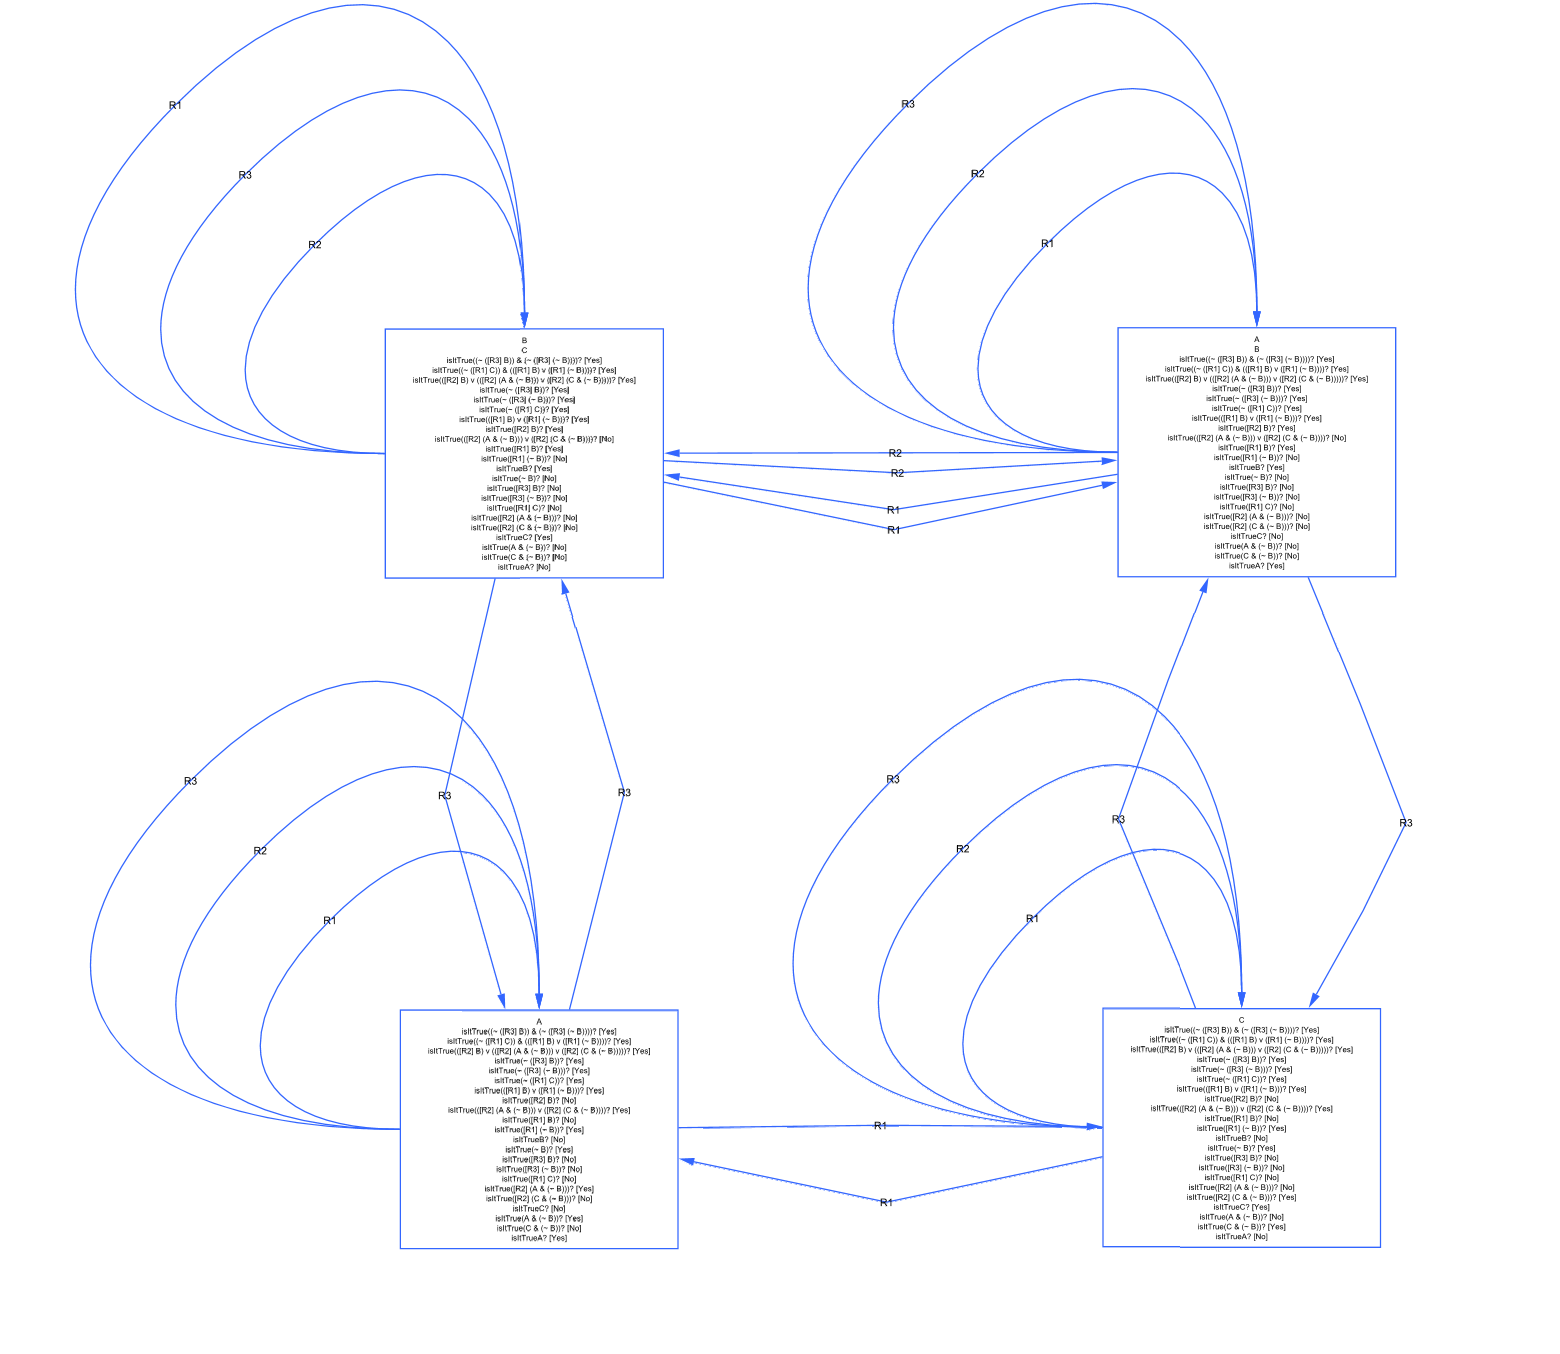
\includegraphics[width=\textwidth]{../premodel_exo4.png}
\caption{Test de validité dans le logiciel LoTREC.}
\label{FigLoTREC}
\end{figure}

\end{document}
